\documentclass[conference]{IEEEtran}
\IEEEoverridecommandlockouts
% The preceding line is only needed to identify funding in the first footnote. If that is unneeded, please comment it out.
\usepackage{cite}
\usepackage{amsmath,amssymb,amsfonts}
\usepackage{algorithmic}
\usepackage{graphicx}
\usepackage{textcomp}
\usepackage{xcolor}
\usepackage{wrapfig}
\usepackage{amssymb}
\usepackage[export]{adjustbox}
\def\BibTeX{{\rm B\kern-.05em{\sc i\kern-.025em b}\kern-.08em
    T\kern-.1667em\lower.7ex\hbox{E}\kern-.125emX}}
\begin{document}

\title{Localization services: GNSS, GPS / A-GPS localization \\
}

\author{\IEEEauthorblockN{1\textsuperscript{st} Gonçalo Couto (up201408558)}
\IEEEauthorblockA{\textit{Dept. Ciência dos Computadores} \\
\textit{FCUP (Universidade do Porto)}\\
\textit{MIERSI}\\
}
\and
\IEEEauthorblockN{2\textsuperscript{nd} Beatriz Saldanha (up201506293)}
\IEEEauthorblockA{\textit{Dept. Ciência dos Computadores} \\
\textit{FCUP (Universidade do Porto)}\\
\textit{MIERSI}\\
}
}

\maketitle

\begin{abstract}

In today's world, localization services have become a hot research topic for a large number of different technologies. The purpose of these technologies is to make life easier for its users, providing a large number of services. In the last years, we've seen the birth of companies that seek to do just that. People can order food, call a taxi or even use these GPS based applications in order to navigate them from, and to, a location. With the creation of smartphones, and smart devices, using these technologies has become simplified, with every phone being able to use them right out of the box. Not only that but, with the developments made to phone bands, A-GPS was made available, this used mobile data connections in order to obtain data in a faster fashion. In the beginning, there was a single GNSS system in use, the United States GPS system, but, in the present time, more countries have developed their own systems. In this paper, we will discuss just how these navigation systems came to be, how they function, and the way they affected human life throughout the years. 

\end{abstract}

\begin{IEEEkeywords}
GNSS, A-GPS, GPS, localization, smartphones, smart devices
\end{IEEEkeywords}

\section{Introduction}
Navigation is defined as the science of getting a craft or person from one place to another[1]. Everyday people around the world do some form of navigation. Going to the store to buy groceries, driving the car to work or even trying to get through those busy and full mall stores during the holidays requires that we have vital navigational traits. Generally, we simply have to use our eyes, common sense or known POI\footnote{Point of interest} in order to get from point A to point B however sometimes that is not enough. Imagine this scenario, you travel overseas, you are in a foreign city and have no knowledge of where you are and want to check a local museum. So, how do you trace your route in order to get to your destination ? This is an example of a situation that happens everyday around the world, with tourists flooding cities. We need a more accurate knowledge of our position. A study conducted by \textit{Riley Panko}[3] with a sample of 500 smartphone users has shown that, over 77\% of these users regularly use navigation apps, with google maps being the dominant choice of all the navigational apps available, which included Waze, Apple Maps, and MapQuest. In 2007, Google launched Street View, a technology that provides interactive panoramas from various positions along many streets in the world. Although, initially only available in the United States, it has expanded to include cities and rural areas worldwide. This is one of the many technologies made available by advancements in the area of navigation.

\begin{figure}
    \centering
    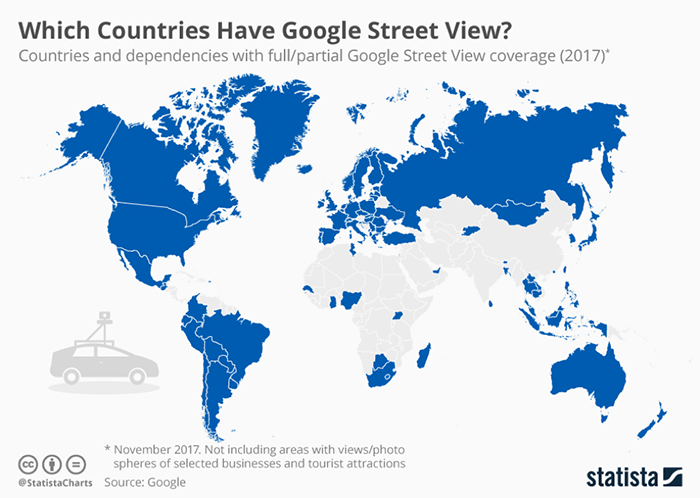
\includegraphics[width=\columnwidth]{countries-with-google-maps.png}
    \caption{World wide street view coverage, November 2017}
\end{figure}

\section{SATNAV Systems}

\subsection{SATNAV Basics}

Satellite navigation or SATNAV, is a system that uses satellites in order to provide autonomous geospatial positioning[2]. It allows small electronic receivers to determine their location (longitude, latitude, and altitude/elevation) to high precision using time signals transmitted along a line of sight by radio from satellites[2]. These kinds of systems can be used for providing position, navigation or for tracking (e.g., something that has been fitted with a receiver). The signals also allow the electronic receiver to calculate the current local time to high precision, which allows time synchronization. SATNAV systems operate independently of any telephonic or internet reception, though these technologies can enhance the usefulness of the positioning information generated[2].

\subsection{SATNAV Today}

Today, there are various SATNAV systems in operation around the globe. Some are global while the others only provide service within certain regions. The term Global Navigation Satellite System (GNSS) is defined as the collection of all SATNAV systems and their augmentations[1].

\section{GNSS}
GNSS is group of SATNAV systems, this means it also functions in a similar way. Given that a person has the required equipment it can provide three-dimensional positioning and velocity information with pinpoint precision continuously. There are core constellations within GNSS which normally consist of 24 or more medium Earth orbit or MEO satellites arranged in 3 or 6 orbital planes with four or more satellites per plane[1]. There are ground monitoring stations that check the "health" and status of the satellites to make sure these are in proper working conditions. These ground stations also upload navigation and other data to the satellites. Since the users of SATNAV systems can only receive data (i.e., the communication is one way only, the receivers do not transmit any data to the satellites) service to an unlimited number of users can be achieved. SATNAV systems use one-way time-of-arrival (TOA) ranging, which requires highly accurate synchronization of sender and receiver clocks. Time-of-arrival measures the time it takes for a signal that was transmitted in a given location to reach a receiver. This time interval is usually referred to as signal propagation time and is then multiplied by the speed of the propagated signal (e.g., speed of light or sound) in order to obtain the distance between the emitter and the receiver. By doing this, and measuring the propagation times of multiple emitters (e.g., navigation equipment) at some given locations, the receiver can determine its position.

\subsection{GLONASS}\label{AA}

GLONASS stands for "Global Navigation Satellite System" and was made in the former U.S.S.R during the mid 1970s. The development of GLONASS was initiated based on former experiences with Doppler satellite Tsikada. The purpose of GLONASS is to provide a continuous service to an unlimited number of users, this service would give them three-dimensional positioning and velocity measures, regardless of weather conditions.
Like many other GNSS systems, GLONASS was intended to be used for military purposes. So with this in mind any land, marine or air type of user could benefit from the service.
GLONASS satellites have circular orbits with an altitude of about 19100km and a period of 11 hours and 15 minutes and 44 seconds. The complete constellation consists of 24 satellites in 3 orbital planes[1].

\subsection{Galileo}

Named after Italian astronomer Galileo Galilei (1564-1642), Galileo is the European contribution to satellite navigation. One of the main objectives of its creation was to make European nations rely less on the U.S. GPS, or the Russian GLONASS as a localization service, due to the fact that these services could be shut down or made unusable by their respective operators at any given time.

\section{GPS}

After the second world war the world was divided into two, east and west. At the east, the communist U.S.S.R or Soviet Union and at the west the democratic, capitalist United States. This conflict became known as the cold war and lasted over 44 years, from 1947 to 1991. During this time there were multiple forms of competition between the two super-powers and one of the most emblematic of them all was the space race, triggered by the launch of Sputnik-1 by the Soviet Union in 1957. This was the first artificial satellite ever launched into the Earth's orbit and the events that followed led to the birth of a GNSS system we use today known as GPS.
During the 1970's, the United States Department of Defense (DoD) wanted a robust, stable satellite navigation system to be available for military purposes that could overcome weaknesses with other navigation methods used at the time.
During the 80's and until the early 90's, a constellation of 24 MEO satellites was launched. Since then, GPS has been a subject to modernization. Civilian use has been authorized since the 1980's.
As with other GNSS systems, GPS satellites operate in six orbital planes at a height of 20.350km and can provide service anywhere on Earth. The orbit time of each satellite is 12 hours and the signal frequency ranges between 1.17645(L1 Band) to 1.57542 GHz(L5 Band).


\subsection{L-Bands}

GPS operates in the L-Band
Frequency spectrum, centered at 1.17645 GHz (L1), 1.22760 GHz (L2), 1.38105 GHz (L3), and 1.57542 GHz (L5).

\subsubsection{Benefits for GPS usage}

\begin{itemize}
    \item L-Bands are able to penetrate clouds, fog, rain, storms and vegetation, this makes the data received by GPS receivers more accurate.
    
    \item Ionospheric delays can be discarded.
    
    \item High bandwidth.
    
    \item Less susceptible to fading due to weather conditions. 
    
\end{itemize}

\subsection{GPS segments}

GPS is broken into three segments: satellite constellation (space segment), ground monitoring and control network (ground segment), and user receiving equipment (user segment). Further elaboration on each of these three areas will be discussed in the next section of this paper.

\subsubsection{\textbf{Space Segment}}

The constellation of satellites from which users make ranging measurements. PRN-coded signals are transmitted from these satellites these signals are then used to make the measurements. Like other GNSS systems GPS is a passive system for the users, this means it transmits the signals and the user passively receives them. Because of this, multiple users can use GPS at the same time. The ranging signal is modulated with information necessary for the receiver to define the satellite's position.

\subsubsection{\textbf{Control Segment}}

The control segment is responsible for maintaining the satellites and to ensure they are in proper working conditions and proper orbital positions. The latter is called station-keeping. The control segment also monitors the satellite solar arrays, battery power levels, and propellant levels used for maneuvers. System availability is also maintained by the control segment as spare satellites are activated if needed. The clock, ephemeris \footnote{The measurement of satellite trajectory.} and almanac \footnote{A subset of ephemeris parameters with reduced precision.} of each satellite is updated at least once a day by the control station, in order to avoid error in data calculations. Several analyses and studies have shown that users benefit from reduced navigation errors with more frequent uploads, thus reducing the upload age of data and accompanying broadcast navigation message errors.[1]

\subsubsection{\textbf{User Segment}}

Consisting of the receiving equipment. This equipment is usually referred to as a GPS receiver, it processes the L-Band signals transmitted by the satellites to determine user PVT. PVT determination is the main use of these devices, although they can be used for other applications such as computing user platform attitude (e.g., heading, pitch and roll) or as a timing source[1].

\begin{figure}
    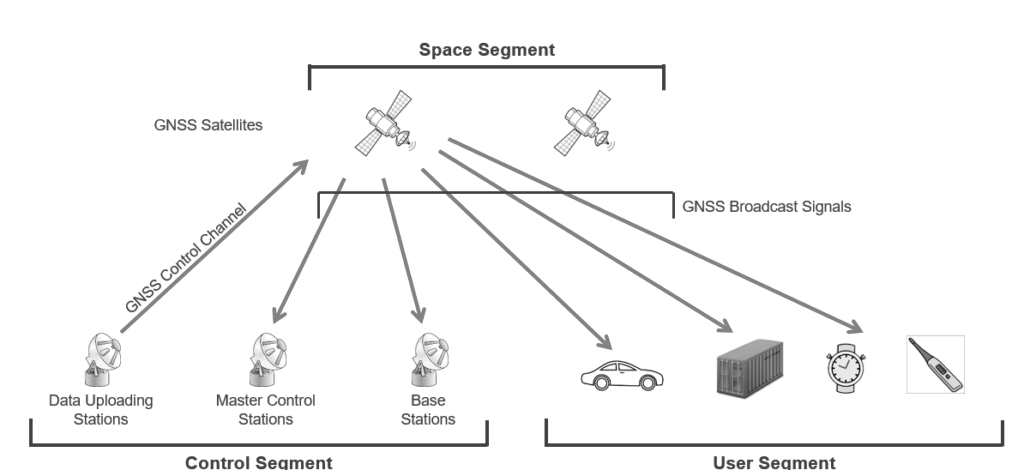
\includegraphics[width=\columnwidth]{img4.png}
    \caption{The different segments of GPS}
\end{figure}

\subsection{GPS Functioning}

In order for the service to operate properly, a GPS receiver must be able to detect at least four of the GPS satellites. These operate according to the following principles[6].

\begin{enumerate}
    \item \textbf{Distance measurement:} A pseudo-noise code is generated by receivers. This code will match the signal coming from the GPS satellite. The signal itself is DSSS (Direct Sequence Spread Spectrum) which means it has been encoded with a chipping sequence. Time offset between locally generated PN sequence and received signal is adjusted until both signals are synchronized. Time offset indicates propagation time from the satellite[6].
    
    \item \textbf{Distance to one satellite:} A certain distance d can be obtained by knowing the speed of electromagnetic propagation between satellites and receiver[6]. 
    
    \item \textbf{Distance to two satellites:} Since the location of two satellites is known, the intersection between the spheres formed by these two satellites forms a circle. The receiver is located anywhere inside this circle[6].
    
    \item \textbf{Distance to three satellites:} Location of the receiver can be one of two possible points of intersection between the three spheres formed by the three satellites. One of the two possible points is usually absurd given the evaluation of longitude, latitude and elevation parameters[6].
    
    \item \textbf{Fourth satellite signal:} Used to detect and correct a timing offset between the GPS clock and the receiver clock[6].
    
\end{enumerate}

\begin{figure}[h!]
    \centering
    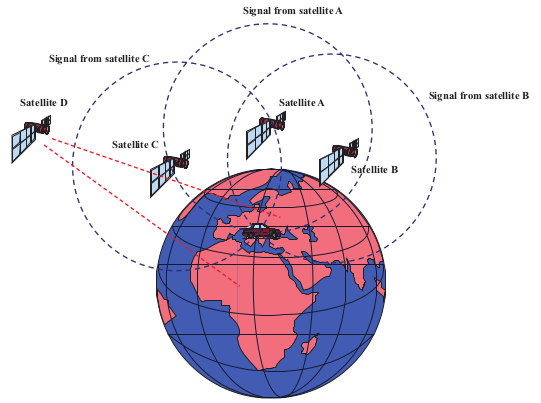
\includegraphics[width=\columnwidth]{img1.png}
    \caption{A visual representation of the process done by GPS receivers[6].}
\end{figure}

\subsection{Time to first fix (TTFF)}

The time required for a GPS receiver to acquire satellite signals and other navigational data (e.g., almanac, ephemeris) in order to calculate a position (a fix).


\subsubsection{\textbf{Cold start}}

The device will try to locate satellites and then calculates a fix, there is no known information since the device has done a dump of all previous data. This process takes the most amount of time.

\subsubsection{\textbf{Warm start}}

The GPS device remembers its last calculated position, almanac, and UTC time data but doesn't know which satellites were in view. It will then perform a reset and try to obtain the satellite signals and then calculates a new position or fix.

\subsubsection{\textbf{Hot start}}

The fastest of the three, the GPS device remembers all previous acquired data (e.g., almanac, UTC time, ephemeris) and attempts to make a fix onto the same satellites and calculate a new position. Generally, this method only works if the device deviates slightly from its last known position before being turned off.

\section{GPS Services}

GPS is a dual-use system. This means it can provide two kinds of separate services, one for civil uses and another for military uses. These two services are known as, Standard Positioning Service (SPS) and Precise Positioning Service (PPS), respectively. SPS is designed for civilian use and, was the predominant satellite navigation service in use by millions of people around the world. PPS is mostly available to the United States military and its allies, for users properly equipped with PPS receivers. Cryptography is used to control access to PPS GPS.

\subsection{SPS - Standard Positioning Service}

SPS provides positioning and timing services, it works only on the L1 signal and uses C/A coding. As said above, its a service fully and freely available to all kinds of users

\subsection{PPS - Precise Positioning Service}

PPS uses a coarse/acquisition (C/A) code ranging signal, with a navigation data message, that is available for peaceful civil, commercial, and scientific use; and a precision (P) code (that will be a Y code) ranging signal with a navigation data message, that is reserved for authorized use[5].
Protection mechanisms where introduced in order to restrict civilian access to full system accuracy, which include:
\bigbreak
\begin{enumerate}

    \item \textbf{Selective Availability or (SA):}
    The purpose of SA is to deny navigation accuracy to potential adversaries by dithering the satellite clock (\(\delta\)-process) or clock degradation, and manipulating the ephemerides (\(\varepsilon\)-process).[GNSS global...] The \(\delta\)-process is done by dithering satellite clock fundamental frequency. Pseudo-range is calculated by comparing the satellite clock and the receiver clock. Since the satellite clock bias has a direct impact on pseudo-range, by doing this, code and carrier pseudo-ranges are affected in the same way.\par
    The (\(\varepsilon\)-process results in the truncation of orbital information that is obtained via the navigation message. Thus, satellite coordinates cannot be accurately computed. Stand-alone receivers are also affected and a similar positioning error occurs.
    
    \begin{figure}[ht]
        \centering
        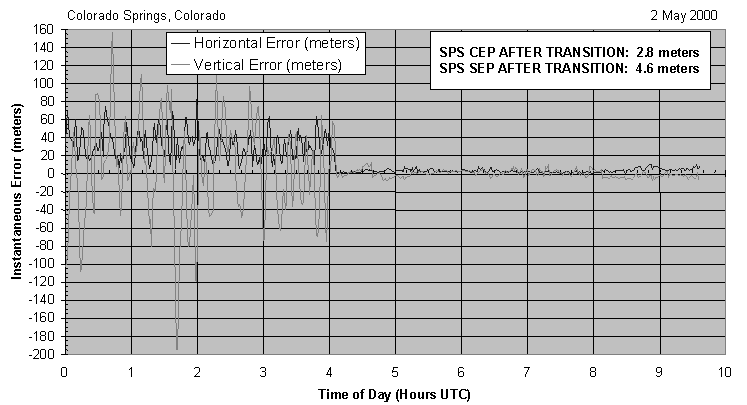
\includegraphics[width=\columnwidth]{fig6.png}
        \caption{GPS accuracy errors before(red) and after(blue) deactivation of SA}
    \end{figure}
    
    \item \textbf{Anti-Spoofing or (AS):}
    Anti-Spoofing is a GPS characteristic that makes it possible to "turn-off" the P-code or use an encrypted code as a way to deny access to the P-code to all but authorized users. The idea behind AS is to keep adversaries from sending fake signals with the GPS signature, in order to create confusion and cause users to misposition themselves.
    AS uses an encrypting W-code to encrypt the P-code, the resulting code is denoted as the Y-code. When AS is active, the P-code on the L1 and L2 carrier is replaced by the unknown Y-code.
    
\end{enumerate}

\section{A-GPS}

A-GPS or Assisted GPS is a performance improvement over the regular GPS. Information is provided through an alternative communications channel (e.g., an antenna or cell tower), instead of the regular way of receiving the signal which is via the satellites themselves.
The task of receiving the signal by the receivers is then simplified, and the amount of time taken to do so minimized.

\begin{figure}
    \centering
    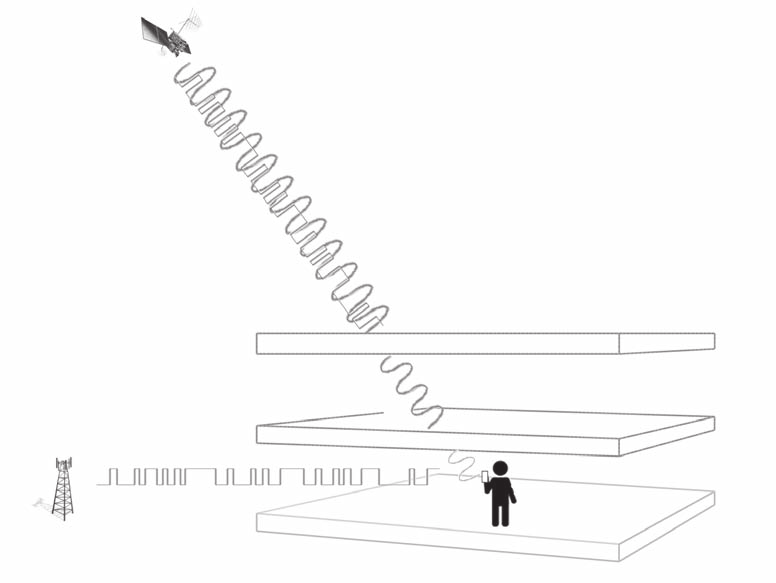
\includegraphics[width=\columnwidth]{img2.png}
    \caption{A-GPS satellite/receiver communication[4]}
\end{figure}

\subsection{A-GPS Functioning}

As explained above one of the key features of A-GPS is that it simplifies and accelerates the process of receiving data by the GPS receiver. It can allow the device to know what frequencies to expect before it even tries, and after this assistance data will provide the satellite positions for use in the GPS computations. Finally, having acquired the satellite signals all that is left to to do is take ranging measurements (this is done in milliseconds, not minutes) and the A-GPS receiver can compute a user's position[4].

\subsection{Modes of operation}

\subsubsection{\textbf{Mobile Station Assisted} (\textbf{MSA)}}

A-GPS device receives data acquisition assistance from a mobile station and an A-GPS server. The position is calculated by the server, and the device only has to capture the data and send the measurements to the mobile station who then uses them with the server.
The A-GPS receiver is helped by a mobile carrier.

\subsubsection{\textbf{Mobile Station Based} (\textbf{MSB)}}

Ephemeris, reference location, timestamp and other optional assistance data are sent to the A-GPS device by the server. With this data sent from the server and the signals received by visible satellites, the device can calculate the position.

\begin{figure}[h]
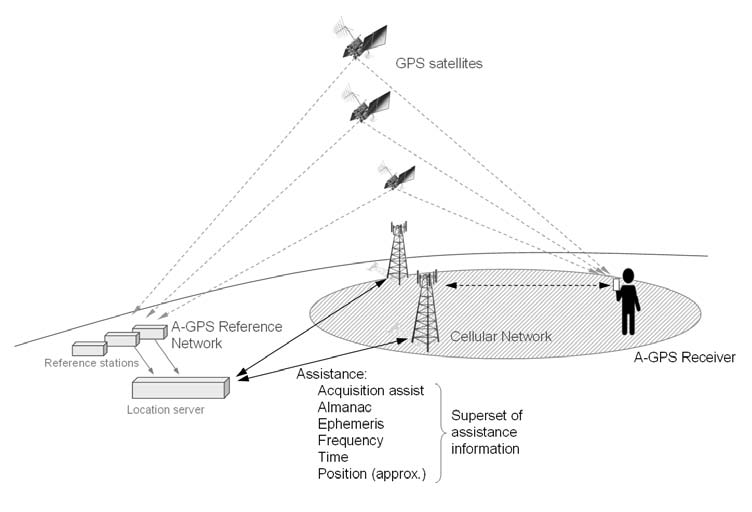
\includegraphics[width=\columnwidth]{img3.png}
    \caption{Illustration of the A-GPS process[4].}
\end{figure}

\section{GPS vs A-GPS}

Regular GPS devices depend only on the information from the satellites. If the signal conditions are poor, the device is not able to fix the position without getting the needed information. Data rates of satellite signals are approximately 50 bit/s, downloading information from the satellites like almanac and ephemeris takes a long time and if the signal is lost the receiver has to start from the beginning.
Assisted GPS fixes this problem due to the fact that the A-GPS receiver can get the information needed from other sources and not the satellite itself. This translates into faster TTFF. Thus improving performance, reliability and giving faster solutions.

\section{Conclusion}

GPS has come a long way since its early years of development and it has revolutionized the surveying and navigation fields. Although originally intended for military uses, its civil applications have grown much faster. Who would have thought that a technology intended to help submarines navigate would become such an important part of human life. Today, anyone that has a smartphone is carrying a portable GPS receiver, and can use this equipment to share location data to other users in order to utilize different types of services. Calling a taxi, tracing routes to a location by using an application (replacing the use of conventional maps), finding nearby restaurants to have dinner, tracking missing persons, etc. The list is endless, and these are things that couldn't be imagined back when the system was first being developed. Some companies are even using the technology to create self-driving vehicles, improving human commodities. In the future, GPS based applications will grow even more and will be limited only to one's imagination.

\begin{thebibliography}{00}
\bibitem{b1} KAPLAN, E. D., J. HEGARTY ed. Understanding GPS/GNSS, Principles and Applications. 3rd ed. London:ARTECH HOUSE, 2017
\bibitem{b2} Wikipedia, "Satelitte Navigation", at wikipedia.org
\bibitem{b3} Riley Panko: "The Popularity of Google Maps: Trends in Navigation Apps in 2018", Jul.2018
\bibitem{b4} DIGGELEN, F., ed. A-GPS: Assisted GPS, GNSS, and SBAS. 1st ed. London:ARTECH HOUSE, 2007
\bibitem{b5} HOFMANN, B. W., LICHTENEGGER, H., WASLE, E ed. GNSS - Global Navigation Satellite Systems, GPS, GLONASS, Galileo and more. 1st ed. New York:Springer, 2008
\bibitem{b6} BEARD, C., W. STALLINGS ed. Wireless Comunication Networks And Systems. 1st ed. New Jersey:Pearson, 2016

\end{thebibliography}

\end{document}
